\documentclass[landscape, a4paper, parskip=half, DIV=13]{scrartcl}
\usepackage[top=1.25cm, bottom=1.0cm, left=7cm, right=7cm, marginparwidth=6.0cm, marginparsep=0pt]{geometry}
\usepackage[dvipsnames]{xcolor}
\usepackage{tikz}
\usetikzlibrary{shapes.geometric}
\usepackage{fontspec}
\usepackage{unicode-math}
\setmainfont{Tex Gyre Schola}
\setmathfont{Tex Gyre Schola Math Regular}
%\setmainfont[Scale=0.95]{Century Gothic}
\usepackage{contour}
\usepackage{multicol}
\setlength{\columnsep}{1cm}
\usepackage{booktabs}
\usepackage{lipsum}
\usepackage{marginnote}
\usepackage{multirow}
\usepackage{enumitem}
\usepackage{embusen}

\setlist[description]{font=\normalfont}

\renewcommand*{\descriptionlabel}[1]{\hspace{\labelsep}\descfont #1:}

%\setkomafont{section}{\setmainfont{Tex Gyre Schola}\Large\textbf}
\setkomafont{section}{\setmainfont[Scale=0.95]{Century Gothic}\LARGE\bfseries}
\setkomafont{subsection}{\setmainfont[Scale=0.95]{Century Gothic}\Large\bfseries}

% Adjust spacing before and after section headings
\RedeclareSectionCommand[
  runin=false,
  beforeskip=1.0\baselineskip,
  afterskip=0.0\baselineskip
]{section}

\RedeclareSectionCommand[
  runin=false,
  beforeskip=0.25\baselineskip,
  afterskip=0.0\baselineskip
]{subsection}

\pagestyle{empty}
\begin{document}
{
%\setmainfont[Scale=2.5]{Tex Gyre Schola}
\setmainfont[Scale=2.5]{Century Gothic}
\begin{center}
\Huge\textbf{\phantom{y}Embusen\phantom{y}}
\end{center}
}
\marginnote{\center
\includegraphics[height=2.375cm]{Images/side_kick_pose.png}\qquad\qquad 
\includegraphics[height=2.5cm]{Images/gedan_burai_pose_left.png}}[-4.125cm]
\reversemarginpar\marginnote{\center
\includegraphics[height=2.5cm]{Images/oi_zuki_pose_right.png}\qquad\qquad \reflectbox{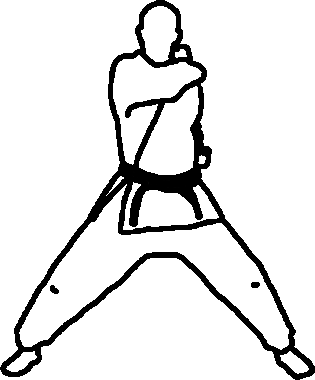
\includegraphics[height=2.5cm]{Images/pinan_sandan_throw_pose.png}}}[-4.125cm]

\vspace{0.0cm}
\vspace{-0.5cm}

\begin{center}
\scalebox{2.88}{
\begin{tikzpicture}

\pic at (0,0in) {kiten={lightgray}};
\pic at (-0.33in, 0in) {gedan_burai={1}};
\pic at (-0.66in, 0in) {chodan_oi_zuki={2}};
\pic[yscale=-1] at (0in, 0in) {chodan_oi_zuki={3}};
\pic[xscale=-1] at (0.33in, 0in) {chodan_oi_zuki={4}};
\pic[rotate=-90] at (0in, 0.33in) {gedan_burai={5}};
\pic[rotate=-90] at (0, 0.66in) {chodan_oi_zuki={6}};
\pic at (0, 0in) {chodan_oi_zuki={7}};
\pic[rotate=90, yscale=-1] at (0, -0.33in) {chodan_oi_zuki={8}};

%\draw[ultra thick, lightgray] (-0.66in, -0.66in) -- (0.33in, -0.66in);
%\draw[ultra thick, lightgray] (0,-0.66in) -- (0, 0.66in);
%\draw[ultra thick, lightgray] (-0.33in, 0.66in) -- (0.66in, 0.66in);

\foreach \i in {-0.99, -0.66, ..., 1.0}
	\foreach \j in {-0.99, -0.88, ..., 1.0} {
		\node[inner sep=0.25pt,fill=gray, circle] at (\i in, \j in) {\phantom{}};
		\node[inner sep=0.25pt,fill=gray, circle] at (\j in, \i in) {\phantom{}};		
}

\foreach \i in {-0.825, -0.495,...,0.826}
	\foreach \j in {-0.825, -0.495,...,0.826}
		\node[inner sep=0.25pt,fill=gray, circle] at (\i in, \j in) {\phantom{}};

%\node[inner sep=0.25pt,fill=black,circle] at (-0.990000in, -0.990000in) {\phantom{}};
%\node[inner sep=0.25pt,fill=black,circle] at (-0.990000in, -0.660000in) {\phantom{}};
%\node[inner sep=0.25pt,fill=black,circle] at (-0.990000in, -0.330000in) {\phantom{}};
%\node[inner sep=0.25pt,fill=black,circle] at (-0.990000in, 0.000000in) {\phantom{}};
%\node[inner sep=0.25pt,fill=black,circle] at (-0.990000in, 0.330000in) {\phantom{}};
%\node[inner sep=0.25pt,fill=black,circle] at (-0.990000in, 0.660000in) {\phantom{}};
%\node[inner sep=0.25pt,fill=black,circle] at (-0.990000in, 0.990000in) {\phantom{}};
%\node[inner sep=0.25pt,fill=black,circle] at (-0.880000in, -0.990000in) {\phantom{}};
%\node[inner sep=0.25pt,fill=black,circle] at (-0.880000in, -0.660000in) {\phantom{}};
%\node[inner sep=0.25pt,fill=black,circle] at (-0.880000in, -0.330000in) {\phantom{}};
%\node[inner sep=0.25pt,fill=black,circle] at (-0.880000in, 0.000000in) {\phantom{}};
%\node[inner sep=0.25pt,fill=black,circle] at (-0.880000in, 0.330000in) {\phantom{}};
%\node[inner sep=0.25pt,fill=black,circle] at (-0.880000in, 0.660000in) {\phantom{}};
%\node[inner sep=0.25pt,fill=black,circle] at (-0.880000in, 0.990000in) {\phantom{}};
%\node[inner sep=0.25pt,fill=black,circle] at (-0.770000in, -0.990000in) {\phantom{}};
%\node[inner sep=0.25pt,fill=black,circle] at (-0.770000in, -0.660000in) {\phantom{}};
%\node[inner sep=0.25pt,fill=black,circle] at (-0.770000in, -0.330000in) {\phantom{}};
%\node[inner sep=0.25pt,fill=black,circle] at (-0.770000in, 0.000000in) {\phantom{}};
%\node[inner sep=0.25pt,fill=black,circle] at (-0.770000in, 0.330000in) {\phantom{}};
%\node[inner sep=0.25pt,fill=black,circle] at (-0.770000in, 0.660000in) {\phantom{}};
%\node[inner sep=0.25pt,fill=black,circle] at (-0.770000in, 0.990000in) {\phantom{}};
%\node[inner sep=0.25pt,fill=black,circle] at (-0.660000in, -0.990000in) {\phantom{}};
%\node[inner sep=0.25pt,fill=black,circle] at (-0.660000in, -0.660000in) {\phantom{}};
%\node[inner sep=0.25pt,fill=black,circle] at (-0.660000in, -0.330000in) {\phantom{}};
%\node[inner sep=0.25pt,fill=black,circle] at (-0.660000in, 0.000000in) {\phantom{}};
%\node[inner sep=0.25pt,fill=black,circle] at (-0.660000in, 0.330000in) {\phantom{}};
%\node[inner sep=0.25pt,fill=black,circle] at (-0.660000in, 0.660000in) {\phantom{}};
%\node[inner sep=0.25pt,fill=black,circle] at (-0.660000in, 0.990000in) {\phantom{}};
%\node[inner sep=0.25pt,fill=black,circle] at (-0.550000in, -0.990000in) {\phantom{}};
%\node[inner sep=0.25pt,fill=black,circle] at (-0.550000in, -0.660000in) {\phantom{}};
%\node[inner sep=0.25pt,fill=black,circle] at (-0.550000in, -0.330000in) {\phantom{}};
%\node[inner sep=0.25pt,fill=black,circle] at (-0.550000in, 0.000000in) {\phantom{}};
%\node[inner sep=0.25pt,fill=black,circle] at (-0.550000in, 0.330000in) {\phantom{}};
%\node[inner sep=0.25pt,fill=black,circle] at (-0.550000in, 0.660000in) {\phantom{}};
%\node[inner sep=0.25pt,fill=black,circle] at (-0.550000in, 0.990000in) {\phantom{}};
%\node[inner sep=0.25pt,fill=black,circle] at (-0.440000in, -0.990000in) {\phantom{}};
%\node[inner sep=0.25pt,fill=black,circle] at (-0.440000in, -0.660000in) {\phantom{}};
%\node[inner sep=0.25pt,fill=black,circle] at (-0.440000in, -0.330000in) {\phantom{}};
%\node[inner sep=0.25pt,fill=black,circle] at (-0.440000in, 0.000000in) {\phantom{}};
%\node[inner sep=0.25pt,fill=black,circle] at (-0.440000in, 0.330000in) {\phantom{}};
%\node[inner sep=0.25pt,fill=black,circle] at (-0.440000in, 0.660000in) {\phantom{}};
%\node[inner sep=0.25pt,fill=black,circle] at (-0.440000in, 0.990000in) {\phantom{}};
%\node[inner sep=0.25pt,fill=black,circle] at (-0.330000in, -0.990000in) {\phantom{}};
%\node[inner sep=0.25pt,fill=black,circle] at (-0.330000in, -0.660000in) {\phantom{}};
%\node[inner sep=0.25pt,fill=black,circle] at (-0.330000in, -0.330000in) {\phantom{}};
%\node[inner sep=0.25pt,fill=black,circle] at (-0.330000in, 0.000000in) {\phantom{}};
%\node[inner sep=0.25pt,fill=black,circle] at (-0.330000in, 0.330000in) {\phantom{}};
%\node[inner sep=0.25pt,fill=black,circle] at (-0.330000in, 0.660000in) {\phantom{}};
%\node[inner sep=0.25pt,fill=black,circle] at (-0.330000in, 0.990000in) {\phantom{}};
%\node[inner sep=0.25pt,fill=black,circle] at (-0.220000in, -0.990000in) {\phantom{}};
%\node[inner sep=0.25pt,fill=black,circle] at (-0.220000in, -0.660000in) {\phantom{}};
%\node[inner sep=0.25pt,fill=black,circle] at (-0.220000in, -0.330000in) {\phantom{}};
%\node[inner sep=0.25pt,fill=black,circle] at (-0.220000in, 0.000000in) {\phantom{}};
%\node[inner sep=0.25pt,fill=black,circle] at (-0.220000in, 0.330000in) {\phantom{}};
%\node[inner sep=0.25pt,fill=black,circle] at (-0.220000in, 0.660000in) {\phantom{}};
%\node[inner sep=0.25pt,fill=black,circle] at (-0.220000in, 0.990000in) {\phantom{}};
%\node[inner sep=0.25pt,fill=black,circle] at (-0.110000in, -0.990000in) {\phantom{}};
%\node[inner sep=0.25pt,fill=black,circle] at (-0.110000in, -0.660000in) {\phantom{}};
%\node[inner sep=0.25pt,fill=black,circle] at (-0.110000in, -0.330000in) {\phantom{}};
%\node[inner sep=0.25pt,fill=black,circle] at (-0.110000in, 0.000000in) {\phantom{}};
%\node[inner sep=0.25pt,fill=black,circle] at (-0.110000in, 0.330000in) {\phantom{}};
%\node[inner sep=0.25pt,fill=black,circle] at (-0.110000in, 0.660000in) {\phantom{}};
%\node[inner sep=0.25pt,fill=black,circle] at (-0.110000in, 0.990000in) {\phantom{}};
%\node[inner sep=0.25pt,fill=black,circle] at (-0.000000in, -0.990000in) {\phantom{}};
%\node[inner sep=0.25pt,fill=black,circle] at (-0.000000in, -0.660000in) {\phantom{}};
%\node[inner sep=0.25pt,fill=black,circle] at (-0.000000in, -0.330000in) {\phantom{}};
%\node[inner sep=0.25pt,fill=black,circle] at (-0.000000in, 0.000000in) {\phantom{}};
%\node[inner sep=0.25pt,fill=black,circle] at (-0.000000in, 0.330000in) {\phantom{}};
%\node[inner sep=0.25pt,fill=black,circle] at (-0.000000in, 0.660000in) {\phantom{}};
%\node[inner sep=0.25pt,fill=black,circle] at (-0.000000in, 0.990000in) {\phantom{}};
%\node[inner sep=0.25pt,fill=black,circle] at (0.110000in, -0.990000in) {\phantom{}};
%\node[inner sep=0.25pt,fill=black,circle] at (0.110000in, -0.660000in) {\phantom{}};
%\node[inner sep=0.25pt,fill=black,circle] at (0.110000in, -0.330000in) {\phantom{}};
%\node[inner sep=0.25pt,fill=black,circle] at (0.110000in, 0.000000in) {\phantom{}};
%\node[inner sep=0.25pt,fill=black,circle] at (0.110000in, 0.330000in) {\phantom{}};
%\node[inner sep=0.25pt,fill=black,circle] at (0.110000in, 0.660000in) {\phantom{}};
%\node[inner sep=0.25pt,fill=black,circle] at (0.110000in, 0.990000in) {\phantom{}};
%\node[inner sep=0.25pt,fill=black,circle] at (0.220000in, -0.990000in) {\phantom{}};
%\node[inner sep=0.25pt,fill=black,circle] at (0.220000in, -0.660000in) {\phantom{}};
%\node[inner sep=0.25pt,fill=black,circle] at (0.220000in, -0.330000in) {\phantom{}};
%\node[inner sep=0.25pt,fill=black,circle] at (0.220000in, 0.000000in) {\phantom{}};
%\node[inner sep=0.25pt,fill=black,circle] at (0.220000in, 0.330000in) {\phantom{}};
%\node[inner sep=0.25pt,fill=black,circle] at (0.220000in, 0.660000in) {\phantom{}};
%\node[inner sep=0.25pt,fill=black,circle] at (0.220000in, 0.990000in) {\phantom{}};
%\node[inner sep=0.25pt,fill=black,circle] at (0.330000in, -0.990000in) {\phantom{}};
%\node[inner sep=0.25pt,fill=black,circle] at (0.330000in, -0.660000in) {\phantom{}};
%\node[inner sep=0.25pt,fill=black,circle] at (0.330000in, -0.330000in) {\phantom{}};
%\node[inner sep=0.25pt,fill=black,circle] at (0.330000in, 0.000000in) {\phantom{}};
%\node[inner sep=0.25pt,fill=black,circle] at (0.330000in, 0.330000in) {\phantom{}};
%\node[inner sep=0.25pt,fill=black,circle] at (0.330000in, 0.660000in) {\phantom{}};
%\node[inner sep=0.25pt,fill=black,circle] at (0.330000in, 0.990000in) {\phantom{}};
%\node[inner sep=0.25pt,fill=black,circle] at (0.440000in, -0.990000in) {\phantom{}};
%\node[inner sep=0.25pt,fill=black,circle] at (0.440000in, -0.660000in) {\phantom{}};
%\node[inner sep=0.25pt,fill=black,circle] at (0.440000in, -0.330000in) {\phantom{}};
%\node[inner sep=0.25pt,fill=black,circle] at (0.440000in, 0.000000in) {\phantom{}};
%\node[inner sep=0.25pt,fill=black,circle] at (0.440000in, 0.330000in) {\phantom{}};
%\node[inner sep=0.25pt,fill=black,circle] at (0.440000in, 0.660000in) {\phantom{}};
%\node[inner sep=0.25pt,fill=black,circle] at (0.440000in, 0.990000in) {\phantom{}};
%\node[inner sep=0.25pt,fill=black,circle] at (0.550000in, -0.990000in) {\phantom{}};
%\node[inner sep=0.25pt,fill=black,circle] at (0.550000in, -0.660000in) {\phantom{}};
%\node[inner sep=0.25pt,fill=black,circle] at (0.550000in, -0.330000in) {\phantom{}};
%\node[inner sep=0.25pt,fill=black,circle] at (0.550000in, 0.000000in) {\phantom{}};
%\node[inner sep=0.25pt,fill=black,circle] at (0.550000in, 0.330000in) {\phantom{}};
%\node[inner sep=0.25pt,fill=black,circle] at (0.550000in, 0.660000in) {\phantom{}};
%\node[inner sep=0.25pt,fill=black,circle] at (0.550000in, 0.990000in) {\phantom{}};
%\node[inner sep=0.25pt,fill=black,circle] at (0.660000in, -0.990000in) {\phantom{}};
%\node[inner sep=0.25pt,fill=black,circle] at (0.660000in, -0.660000in) {\phantom{}};
%\node[inner sep=0.25pt,fill=black,circle] at (0.660000in, -0.330000in) {\phantom{}};
%\node[inner sep=0.25pt,fill=black,circle] at (0.660000in, 0.000000in) {\phantom{}};
%\node[inner sep=0.25pt,fill=black,circle] at (0.660000in, 0.330000in) {\phantom{}};
%\node[inner sep=0.25pt,fill=black,circle] at (0.660000in, 0.660000in) {\phantom{}};
%\node[inner sep=0.25pt,fill=black,circle] at (0.660000in, 0.990000in) {\phantom{}};
%\node[inner sep=0.25pt,fill=black,circle] at (0.770000in, -0.990000in) {\phantom{}};
%\node[inner sep=0.25pt,fill=black,circle] at (0.770000in, -0.660000in) {\phantom{}};
%\node[inner sep=0.25pt,fill=black,circle] at (0.770000in, -0.330000in) {\phantom{}};
%\node[inner sep=0.25pt,fill=black,circle] at (0.770000in, 0.000000in) {\phantom{}};
%\node[inner sep=0.25pt,fill=black,circle] at (0.770000in, 0.330000in) {\phantom{}};
%\node[inner sep=0.25pt,fill=black,circle] at (0.770000in, 0.660000in) {\phantom{}};
%\node[inner sep=0.25pt,fill=black,circle] at (0.770000in, 0.990000in) {\phantom{}};
%\node[inner sep=0.25pt,fill=black,circle] at (0.880000in, -0.990000in) {\phantom{}};
%\node[inner sep=0.25pt,fill=black,circle] at (0.880000in, -0.660000in) {\phantom{}};
%\node[inner sep=0.25pt,fill=black,circle] at (0.880000in, -0.330000in) {\phantom{}};
%\node[inner sep=0.25pt,fill=black,circle] at (0.880000in, 0.000000in) {\phantom{}};
%\node[inner sep=0.25pt,fill=black,circle] at (0.880000in, 0.330000in) {\phantom{}};
%\node[inner sep=0.25pt,fill=black,circle] at (0.880000in, 0.660000in) {\phantom{}};
%\node[inner sep=0.25pt,fill=black,circle] at (0.880000in, 0.990000in) {\phantom{}};
%\node[inner sep=0.25pt,fill=black,circle] at (0.990000in, -0.990000in) {\phantom{}};
%\node[inner sep=0.25pt,fill=black,circle] at (0.990000in, -0.660000in) {\phantom{}};
%\node[inner sep=0.25pt,fill=black,circle] at (0.990000in, -0.330000in) {\phantom{}};
%\node[inner sep=0.25pt,fill=black,circle] at (0.990000in, 0.000000in) {\phantom{}};
%\node[inner sep=0.25pt,fill=black,circle] at (0.990000in, 0.330000in) {\phantom{}};
%\node[inner sep=0.25pt,fill=black,circle] at (0.990000in, 0.660000in) {\phantom{}};
%\node[inner sep=0.25pt,fill=black,circle] at (0.990000in, 0.990000in) {\phantom{}};
%\node[inner sep=0.25pt,fill=black,circle] at (-0.990000in, -0.990000in) {\phantom{}};
%\node[inner sep=0.25pt,fill=black,circle] at (-0.990000in, -0.880000in) {\phantom{}};
%\node[inner sep=0.25pt,fill=black,circle] at (-0.990000in, -0.770000in) {\phantom{}};
%\node[inner sep=0.25pt,fill=black,circle] at (-0.990000in, -0.660000in) {\phantom{}};
%\node[inner sep=0.25pt,fill=black,circle] at (-0.990000in, -0.550000in) {\phantom{}};
%\node[inner sep=0.25pt,fill=black,circle] at (-0.990000in, -0.440000in) {\phantom{}};
%\node[inner sep=0.25pt,fill=black,circle] at (-0.990000in, -0.330000in) {\phantom{}};
%\node[inner sep=0.25pt,fill=black,circle] at (-0.990000in, -0.220000in) {\phantom{}};
%\node[inner sep=0.25pt,fill=black,circle] at (-0.990000in, -0.110000in) {\phantom{}};
%\node[inner sep=0.25pt,fill=black,circle] at (-0.990000in, -0.000000in) {\phantom{}};
%\node[inner sep=0.25pt,fill=black,circle] at (-0.990000in, 0.110000in) {\phantom{}};
%\node[inner sep=0.25pt,fill=black,circle] at (-0.990000in, 0.220000in) {\phantom{}};
%\node[inner sep=0.25pt,fill=black,circle] at (-0.990000in, 0.330000in) {\phantom{}};
%\node[inner sep=0.25pt,fill=black,circle] at (-0.990000in, 0.440000in) {\phantom{}};
%\node[inner sep=0.25pt,fill=black,circle] at (-0.990000in, 0.550000in) {\phantom{}};
%\node[inner sep=0.25pt,fill=black,circle] at (-0.990000in, 0.660000in) {\phantom{}};
%\node[inner sep=0.25pt,fill=black,circle] at (-0.990000in, 0.770000in) {\phantom{}};
%\node[inner sep=0.25pt,fill=black,circle] at (-0.990000in, 0.880000in) {\phantom{}};
%\node[inner sep=0.25pt,fill=black,circle] at (-0.990000in, 0.990000in) {\phantom{}};
%\node[inner sep=0.25pt,fill=black,circle] at (-0.660000in, -0.990000in) {\phantom{}};
%\node[inner sep=0.25pt,fill=black,circle] at (-0.660000in, -0.880000in) {\phantom{}};
%\node[inner sep=0.25pt,fill=black,circle] at (-0.660000in, -0.770000in) {\phantom{}};
%\node[inner sep=0.25pt,fill=black,circle] at (-0.660000in, -0.660000in) {\phantom{}};
%\node[inner sep=0.25pt,fill=black,circle] at (-0.660000in, -0.550000in) {\phantom{}};
%\node[inner sep=0.25pt,fill=black,circle] at (-0.660000in, -0.440000in) {\phantom{}};
%\node[inner sep=0.25pt,fill=black,circle] at (-0.660000in, -0.330000in) {\phantom{}};
%\node[inner sep=0.25pt,fill=black,circle] at (-0.660000in, -0.220000in) {\phantom{}};
%\node[inner sep=0.25pt,fill=black,circle] at (-0.660000in, -0.110000in) {\phantom{}};
%\node[inner sep=0.25pt,fill=black,circle] at (-0.660000in, -0.000000in) {\phantom{}};
%\node[inner sep=0.25pt,fill=black,circle] at (-0.660000in, 0.110000in) {\phantom{}};
%\node[inner sep=0.25pt,fill=black,circle] at (-0.660000in, 0.220000in) {\phantom{}};
%\node[inner sep=0.25pt,fill=black,circle] at (-0.660000in, 0.330000in) {\phantom{}};
%\node[inner sep=0.25pt,fill=black,circle] at (-0.660000in, 0.440000in) {\phantom{}};
%\node[inner sep=0.25pt,fill=black,circle] at (-0.660000in, 0.550000in) {\phantom{}};
%\node[inner sep=0.25pt,fill=black,circle] at (-0.660000in, 0.660000in) {\phantom{}};
%\node[inner sep=0.25pt,fill=black,circle] at (-0.660000in, 0.770000in) {\phantom{}};
%\node[inner sep=0.25pt,fill=black,circle] at (-0.660000in, 0.880000in) {\phantom{}};
%\node[inner sep=0.25pt,fill=black,circle] at (-0.660000in, 0.990000in) {\phantom{}};
%\node[inner sep=0.25pt,fill=black,circle] at (-0.330000in, -0.990000in) {\phantom{}};
%\node[inner sep=0.25pt,fill=black,circle] at (-0.330000in, -0.880000in) {\phantom{}};
%\node[inner sep=0.25pt,fill=black,circle] at (-0.330000in, -0.770000in) {\phantom{}};
%\node[inner sep=0.25pt,fill=black,circle] at (-0.330000in, -0.660000in) {\phantom{}};
%\node[inner sep=0.25pt,fill=black,circle] at (-0.330000in, -0.550000in) {\phantom{}};
%\node[inner sep=0.25pt,fill=black,circle] at (-0.330000in, -0.440000in) {\phantom{}};
%\node[inner sep=0.25pt,fill=black,circle] at (-0.330000in, -0.330000in) {\phantom{}};
%\node[inner sep=0.25pt,fill=black,circle] at (-0.330000in, -0.220000in) {\phantom{}};
%\node[inner sep=0.25pt,fill=black,circle] at (-0.330000in, -0.110000in) {\phantom{}};
%\node[inner sep=0.25pt,fill=black,circle] at (-0.330000in, -0.000000in) {\phantom{}};
%\node[inner sep=0.25pt,fill=black,circle] at (-0.330000in, 0.110000in) {\phantom{}};
%\node[inner sep=0.25pt,fill=black,circle] at (-0.330000in, 0.220000in) {\phantom{}};
%\node[inner sep=0.25pt,fill=black,circle] at (-0.330000in, 0.330000in) {\phantom{}};
%\node[inner sep=0.25pt,fill=black,circle] at (-0.330000in, 0.440000in) {\phantom{}};
%\node[inner sep=0.25pt,fill=black,circle] at (-0.330000in, 0.550000in) {\phantom{}};
%\node[inner sep=0.25pt,fill=black,circle] at (-0.330000in, 0.660000in) {\phantom{}};
%\node[inner sep=0.25pt,fill=black,circle] at (-0.330000in, 0.770000in) {\phantom{}};
%\node[inner sep=0.25pt,fill=black,circle] at (-0.330000in, 0.880000in) {\phantom{}};
%\node[inner sep=0.25pt,fill=black,circle] at (-0.330000in, 0.990000in) {\phantom{}};
%\node[inner sep=0.25pt,fill=black,circle] at (0.000000in, -0.990000in) {\phantom{}};
%\node[inner sep=0.25pt,fill=black,circle] at (0.000000in, -0.880000in) {\phantom{}};
%\node[inner sep=0.25pt,fill=black,circle] at (0.000000in, -0.770000in) {\phantom{}};
%\node[inner sep=0.25pt,fill=black,circle] at (0.000000in, -0.660000in) {\phantom{}};
%\node[inner sep=0.25pt,fill=black,circle] at (0.000000in, -0.550000in) {\phantom{}};
%\node[inner sep=0.25pt,fill=black,circle] at (0.000000in, -0.440000in) {\phantom{}};
%\node[inner sep=0.25pt,fill=black,circle] at (0.000000in, -0.330000in) {\phantom{}};
%\node[inner sep=0.25pt,fill=black,circle] at (0.000000in, -0.220000in) {\phantom{}};
%\node[inner sep=0.25pt,fill=black,circle] at (0.000000in, -0.110000in) {\phantom{}};
%\node[inner sep=0.25pt,fill=black,circle] at (0.000000in, -0.000000in) {\phantom{}};
%\node[inner sep=0.25pt,fill=black,circle] at (0.000000in, 0.110000in) {\phantom{}};
%\node[inner sep=0.25pt,fill=black,circle] at (0.000000in, 0.220000in) {\phantom{}};
%\node[inner sep=0.25pt,fill=black,circle] at (0.000000in, 0.330000in) {\phantom{}};
%\node[inner sep=0.25pt,fill=black,circle] at (0.000000in, 0.440000in) {\phantom{}};
%\node[inner sep=0.25pt,fill=black,circle] at (0.000000in, 0.550000in) {\phantom{}};
%\node[inner sep=0.25pt,fill=black,circle] at (0.000000in, 0.660000in) {\phantom{}};
%\node[inner sep=0.25pt,fill=black,circle] at (0.000000in, 0.770000in) {\phantom{}};
%\node[inner sep=0.25pt,fill=black,circle] at (0.000000in, 0.880000in) {\phantom{}};
%\node[inner sep=0.25pt,fill=black,circle] at (0.000000in, 0.990000in) {\phantom{}};
%\node[inner sep=0.25pt,fill=black,circle] at (0.330000in, -0.990000in) {\phantom{}};
%\node[inner sep=0.25pt,fill=black,circle] at (0.330000in, -0.880000in) {\phantom{}};
%\node[inner sep=0.25pt,fill=black,circle] at (0.330000in, -0.770000in) {\phantom{}};
%\node[inner sep=0.25pt,fill=black,circle] at (0.330000in, -0.660000in) {\phantom{}};
%\node[inner sep=0.25pt,fill=black,circle] at (0.330000in, -0.550000in) {\phantom{}};
%\node[inner sep=0.25pt,fill=black,circle] at (0.330000in, -0.440000in) {\phantom{}};
%\node[inner sep=0.25pt,fill=black,circle] at (0.330000in, -0.330000in) {\phantom{}};
%\node[inner sep=0.25pt,fill=black,circle] at (0.330000in, -0.220000in) {\phantom{}};
%\node[inner sep=0.25pt,fill=black,circle] at (0.330000in, -0.110000in) {\phantom{}};
%\node[inner sep=0.25pt,fill=black,circle] at (0.330000in, -0.000000in) {\phantom{}};
%\node[inner sep=0.25pt,fill=black,circle] at (0.330000in, 0.110000in) {\phantom{}};
%\node[inner sep=0.25pt,fill=black,circle] at (0.330000in, 0.220000in) {\phantom{}};
%\node[inner sep=0.25pt,fill=black,circle] at (0.330000in, 0.330000in) {\phantom{}};
%\node[inner sep=0.25pt,fill=black,circle] at (0.330000in, 0.440000in) {\phantom{}};
%\node[inner sep=0.25pt,fill=black,circle] at (0.330000in, 0.550000in) {\phantom{}};
%\node[inner sep=0.25pt,fill=black,circle] at (0.330000in, 0.660000in) {\phantom{}};
%\node[inner sep=0.25pt,fill=black,circle] at (0.330000in, 0.770000in) {\phantom{}};
%\node[inner sep=0.25pt,fill=black,circle] at (0.330000in, 0.880000in) {\phantom{}};
%\node[inner sep=0.25pt,fill=black,circle] at (0.330000in, 0.990000in) {\phantom{}};
%\node[inner sep=0.25pt,fill=black,circle] at (0.660000in, -0.990000in) {\phantom{}};
%\node[inner sep=0.25pt,fill=black,circle] at (0.660000in, -0.880000in) {\phantom{}};
%\node[inner sep=0.25pt,fill=black,circle] at (0.660000in, -0.770000in) {\phantom{}};
%\node[inner sep=0.25pt,fill=black,circle] at (0.660000in, -0.660000in) {\phantom{}};
%\node[inner sep=0.25pt,fill=black,circle] at (0.660000in, -0.550000in) {\phantom{}};
%\node[inner sep=0.25pt,fill=black,circle] at (0.660000in, -0.440000in) {\phantom{}};
%\node[inner sep=0.25pt,fill=black,circle] at (0.660000in, -0.330000in) {\phantom{}};
%\node[inner sep=0.25pt,fill=black,circle] at (0.660000in, -0.220000in) {\phantom{}};
%\node[inner sep=0.25pt,fill=black,circle] at (0.660000in, -0.110000in) {\phantom{}};
%\node[inner sep=0.25pt,fill=black,circle] at (0.660000in, -0.000000in) {\phantom{}};
%\node[inner sep=0.25pt,fill=black,circle] at (0.660000in, 0.110000in) {\phantom{}};
%\node[inner sep=0.25pt,fill=black,circle] at (0.660000in, 0.220000in) {\phantom{}};
%\node[inner sep=0.25pt,fill=black,circle] at (0.660000in, 0.330000in) {\phantom{}};
%\node[inner sep=0.25pt,fill=black,circle] at (0.660000in, 0.440000in) {\phantom{}};
%\node[inner sep=0.25pt,fill=black,circle] at (0.660000in, 0.550000in) {\phantom{}};
%\node[inner sep=0.25pt,fill=black,circle] at (0.660000in, 0.660000in) {\phantom{}};
%\node[inner sep=0.25pt,fill=black,circle] at (0.660000in, 0.770000in) {\phantom{}};
%\node[inner sep=0.25pt,fill=black,circle] at (0.660000in, 0.880000in) {\phantom{}};
%\node[inner sep=0.25pt,fill=black,circle] at (0.660000in, 0.990000in) {\phantom{}};
%\node[inner sep=0.25pt,fill=black,circle] at (0.990000in, -0.990000in) {\phantom{}};
%\node[inner sep=0.25pt,fill=black,circle] at (0.990000in, -0.880000in) {\phantom{}};
%\node[inner sep=0.25pt,fill=black,circle] at (0.990000in, -0.770000in) {\phantom{}};
%\node[inner sep=0.25pt,fill=black,circle] at (0.990000in, -0.660000in) {\phantom{}};
%\node[inner sep=0.25pt,fill=black,circle] at (0.990000in, -0.550000in) {\phantom{}};
%\node[inner sep=0.25pt,fill=black,circle] at (0.990000in, -0.440000in) {\phantom{}};
%\node[inner sep=0.25pt,fill=black,circle] at (0.990000in, -0.330000in) {\phantom{}};
%\node[inner sep=0.25pt,fill=black,circle] at (0.990000in, -0.220000in) {\phantom{}};
%\node[inner sep=0.25pt,fill=black,circle] at (0.990000in, -0.110000in) {\phantom{}};
%\node[inner sep=0.25pt,fill=black,circle] at (0.990000in, -0.000000in) {\phantom{}};
%\node[inner sep=0.25pt,fill=black,circle] at (0.990000in, 0.110000in) {\phantom{}};
%\node[inner sep=0.25pt,fill=black,circle] at (0.990000in, 0.220000in) {\phantom{}};
%\node[inner sep=0.25pt,fill=black,circle] at (0.990000in, 0.330000in) {\phantom{}};
%\node[inner sep=0.25pt,fill=black,circle] at (0.990000in, 0.440000in) {\phantom{}};
%\node[inner sep=0.25pt,fill=black,circle] at (0.990000in, 0.550000in) {\phantom{}};
%\node[inner sep=0.25pt,fill=black,circle] at (0.990000in, 0.660000in) {\phantom{}};
%\node[inner sep=0.25pt,fill=black,circle] at (0.990000in, 0.770000in) {\phantom{}};
%\node[inner sep=0.25pt,fill=black,circle] at (0.990000in, 0.880000in) {\phantom{}};
%\node[inner sep=0.25pt,fill=black,circle] at (0.990000in, 0.990000in) {\phantom{}};
\node[draw,line width=0.25mm,minimum width=1.99in,minimum height=1.99in] at (0in,0in) {\phantom{}};
\end{tikzpicture}
%\begin{tikzpicture}

\pic at (0,-0.66in) {kiten={lightgray}};
\pic at (-0.33in, -0.66in) {gedan_burai={1/17\ \ \ \ }};
\pic at (-0.66in, -0.66in) {chodan_oi_zuki={2/18\ \ \ \ }};
\pic[xscale=-1] at (0in, -0.66in) {gedan_burai={\ \ \ \ 3/19}};
\pic[xscale=-1] at (0.33in, -0.66in) {chodan_oi_zuki={\ \ \ 4/20}};
\pic[rotate=-90] at (0in, -0.33in) {gedan_burai={5}};
\pic[rotate=-90] at (0, 0) {chodan_oi_zuki={6}};
\pic[rotate=-90, yscale=-1] at (0, 0.33in) {chodan_oi_zuki={7}};
\pic[rotate=-90] at (0, 0.66in) {chodan_oi_zuki={8}};
\pic[rotate=180] at (0.33in, 0.66in) {gedan_burai={9}};
\pic[rotate=180] at (0.66in, 0.66in) {chodan_oi_zuki={10}};
\pic[yscale=-1] at (0in, 0.66in) {gedan_burai={11}};
\pic[yscale=-1] at (-0.33in, 0.66in) {chodan_oi_zuki={12}};
\pic[rotate=90] at (0, 0.33in) {gedan_burai={13}};
\pic[rotate=90] at (0, 0) {chodan_oi_zuki={14}};
\pic[rotate=90, yscale=-1] at (0, -0.33in) {chodan_oi_zuki={15}};
\pic[rotate=90] at (0, -0.66in) {chodan_oi_zuki={16}};

%\draw[ultra thick, lightgray] (-0.66in, -0.66in) -- (0.33in, -0.66in);
%\draw[ultra thick, lightgray] (0,-0.66in) -- (0, 0.66in);
%\draw[ultra thick, lightgray] (-0.33in, 0.66in) -- (0.66in, 0.66in);

\foreach \i in {-0.99, -0.66, ..., 1.0}
	\foreach \j in {-0.99, -0.88, ..., 1.0} {
		\node[inner sep=0.25pt,fill=gray, circle] at (\i in, \j in) {\phantom{}};
		\node[inner sep=0.25pt,fill=gray, circle] at (\j in, \i in) {\phantom{}};		
}

\foreach \i in {-0.825, -0.495,...,0.826}
	\foreach \j in {-0.825, -0.495,...,0.826}
		\node[inner sep=0.25pt,fill=gray, circle] at (\i in, \j in) {\phantom{}};

%\node[inner sep=0.25pt,fill=black,circle] at (-0.990000in, -0.990000in) {\phantom{}};
%\node[inner sep=0.25pt,fill=black,circle] at (-0.990000in, -0.660000in) {\phantom{}};
%\node[inner sep=0.25pt,fill=black,circle] at (-0.990000in, -0.330000in) {\phantom{}};
%\node[inner sep=0.25pt,fill=black,circle] at (-0.990000in, 0.000000in) {\phantom{}};
%\node[inner sep=0.25pt,fill=black,circle] at (-0.990000in, 0.330000in) {\phantom{}};
%\node[inner sep=0.25pt,fill=black,circle] at (-0.990000in, 0.660000in) {\phantom{}};
%\node[inner sep=0.25pt,fill=black,circle] at (-0.990000in, 0.990000in) {\phantom{}};
%\node[inner sep=0.25pt,fill=black,circle] at (-0.880000in, -0.990000in) {\phantom{}};
%\node[inner sep=0.25pt,fill=black,circle] at (-0.880000in, -0.660000in) {\phantom{}};
%\node[inner sep=0.25pt,fill=black,circle] at (-0.880000in, -0.330000in) {\phantom{}};
%\node[inner sep=0.25pt,fill=black,circle] at (-0.880000in, 0.000000in) {\phantom{}};
%\node[inner sep=0.25pt,fill=black,circle] at (-0.880000in, 0.330000in) {\phantom{}};
%\node[inner sep=0.25pt,fill=black,circle] at (-0.880000in, 0.660000in) {\phantom{}};
%\node[inner sep=0.25pt,fill=black,circle] at (-0.880000in, 0.990000in) {\phantom{}};
%\node[inner sep=0.25pt,fill=black,circle] at (-0.770000in, -0.990000in) {\phantom{}};
%\node[inner sep=0.25pt,fill=black,circle] at (-0.770000in, -0.660000in) {\phantom{}};
%\node[inner sep=0.25pt,fill=black,circle] at (-0.770000in, -0.330000in) {\phantom{}};
%\node[inner sep=0.25pt,fill=black,circle] at (-0.770000in, 0.000000in) {\phantom{}};
%\node[inner sep=0.25pt,fill=black,circle] at (-0.770000in, 0.330000in) {\phantom{}};
%\node[inner sep=0.25pt,fill=black,circle] at (-0.770000in, 0.660000in) {\phantom{}};
%\node[inner sep=0.25pt,fill=black,circle] at (-0.770000in, 0.990000in) {\phantom{}};
%\node[inner sep=0.25pt,fill=black,circle] at (-0.660000in, -0.990000in) {\phantom{}};
%\node[inner sep=0.25pt,fill=black,circle] at (-0.660000in, -0.660000in) {\phantom{}};
%\node[inner sep=0.25pt,fill=black,circle] at (-0.660000in, -0.330000in) {\phantom{}};
%\node[inner sep=0.25pt,fill=black,circle] at (-0.660000in, 0.000000in) {\phantom{}};
%\node[inner sep=0.25pt,fill=black,circle] at (-0.660000in, 0.330000in) {\phantom{}};
%\node[inner sep=0.25pt,fill=black,circle] at (-0.660000in, 0.660000in) {\phantom{}};
%\node[inner sep=0.25pt,fill=black,circle] at (-0.660000in, 0.990000in) {\phantom{}};
%\node[inner sep=0.25pt,fill=black,circle] at (-0.550000in, -0.990000in) {\phantom{}};
%\node[inner sep=0.25pt,fill=black,circle] at (-0.550000in, -0.660000in) {\phantom{}};
%\node[inner sep=0.25pt,fill=black,circle] at (-0.550000in, -0.330000in) {\phantom{}};
%\node[inner sep=0.25pt,fill=black,circle] at (-0.550000in, 0.000000in) {\phantom{}};
%\node[inner sep=0.25pt,fill=black,circle] at (-0.550000in, 0.330000in) {\phantom{}};
%\node[inner sep=0.25pt,fill=black,circle] at (-0.550000in, 0.660000in) {\phantom{}};
%\node[inner sep=0.25pt,fill=black,circle] at (-0.550000in, 0.990000in) {\phantom{}};
%\node[inner sep=0.25pt,fill=black,circle] at (-0.440000in, -0.990000in) {\phantom{}};
%\node[inner sep=0.25pt,fill=black,circle] at (-0.440000in, -0.660000in) {\phantom{}};
%\node[inner sep=0.25pt,fill=black,circle] at (-0.440000in, -0.330000in) {\phantom{}};
%\node[inner sep=0.25pt,fill=black,circle] at (-0.440000in, 0.000000in) {\phantom{}};
%\node[inner sep=0.25pt,fill=black,circle] at (-0.440000in, 0.330000in) {\phantom{}};
%\node[inner sep=0.25pt,fill=black,circle] at (-0.440000in, 0.660000in) {\phantom{}};
%\node[inner sep=0.25pt,fill=black,circle] at (-0.440000in, 0.990000in) {\phantom{}};
%\node[inner sep=0.25pt,fill=black,circle] at (-0.330000in, -0.990000in) {\phantom{}};
%\node[inner sep=0.25pt,fill=black,circle] at (-0.330000in, -0.660000in) {\phantom{}};
%\node[inner sep=0.25pt,fill=black,circle] at (-0.330000in, -0.330000in) {\phantom{}};
%\node[inner sep=0.25pt,fill=black,circle] at (-0.330000in, 0.000000in) {\phantom{}};
%\node[inner sep=0.25pt,fill=black,circle] at (-0.330000in, 0.330000in) {\phantom{}};
%\node[inner sep=0.25pt,fill=black,circle] at (-0.330000in, 0.660000in) {\phantom{}};
%\node[inner sep=0.25pt,fill=black,circle] at (-0.330000in, 0.990000in) {\phantom{}};
%\node[inner sep=0.25pt,fill=black,circle] at (-0.220000in, -0.990000in) {\phantom{}};
%\node[inner sep=0.25pt,fill=black,circle] at (-0.220000in, -0.660000in) {\phantom{}};
%\node[inner sep=0.25pt,fill=black,circle] at (-0.220000in, -0.330000in) {\phantom{}};
%\node[inner sep=0.25pt,fill=black,circle] at (-0.220000in, 0.000000in) {\phantom{}};
%\node[inner sep=0.25pt,fill=black,circle] at (-0.220000in, 0.330000in) {\phantom{}};
%\node[inner sep=0.25pt,fill=black,circle] at (-0.220000in, 0.660000in) {\phantom{}};
%\node[inner sep=0.25pt,fill=black,circle] at (-0.220000in, 0.990000in) {\phantom{}};
%\node[inner sep=0.25pt,fill=black,circle] at (-0.110000in, -0.990000in) {\phantom{}};
%\node[inner sep=0.25pt,fill=black,circle] at (-0.110000in, -0.660000in) {\phantom{}};
%\node[inner sep=0.25pt,fill=black,circle] at (-0.110000in, -0.330000in) {\phantom{}};
%\node[inner sep=0.25pt,fill=black,circle] at (-0.110000in, 0.000000in) {\phantom{}};
%\node[inner sep=0.25pt,fill=black,circle] at (-0.110000in, 0.330000in) {\phantom{}};
%\node[inner sep=0.25pt,fill=black,circle] at (-0.110000in, 0.660000in) {\phantom{}};
%\node[inner sep=0.25pt,fill=black,circle] at (-0.110000in, 0.990000in) {\phantom{}};
%\node[inner sep=0.25pt,fill=black,circle] at (-0.000000in, -0.990000in) {\phantom{}};
%\node[inner sep=0.25pt,fill=black,circle] at (-0.000000in, -0.660000in) {\phantom{}};
%\node[inner sep=0.25pt,fill=black,circle] at (-0.000000in, -0.330000in) {\phantom{}};
%\node[inner sep=0.25pt,fill=black,circle] at (-0.000000in, 0.000000in) {\phantom{}};
%\node[inner sep=0.25pt,fill=black,circle] at (-0.000000in, 0.330000in) {\phantom{}};
%\node[inner sep=0.25pt,fill=black,circle] at (-0.000000in, 0.660000in) {\phantom{}};
%\node[inner sep=0.25pt,fill=black,circle] at (-0.000000in, 0.990000in) {\phantom{}};
%\node[inner sep=0.25pt,fill=black,circle] at (0.110000in, -0.990000in) {\phantom{}};
%\node[inner sep=0.25pt,fill=black,circle] at (0.110000in, -0.660000in) {\phantom{}};
%\node[inner sep=0.25pt,fill=black,circle] at (0.110000in, -0.330000in) {\phantom{}};
%\node[inner sep=0.25pt,fill=black,circle] at (0.110000in, 0.000000in) {\phantom{}};
%\node[inner sep=0.25pt,fill=black,circle] at (0.110000in, 0.330000in) {\phantom{}};
%\node[inner sep=0.25pt,fill=black,circle] at (0.110000in, 0.660000in) {\phantom{}};
%\node[inner sep=0.25pt,fill=black,circle] at (0.110000in, 0.990000in) {\phantom{}};
%\node[inner sep=0.25pt,fill=black,circle] at (0.220000in, -0.990000in) {\phantom{}};
%\node[inner sep=0.25pt,fill=black,circle] at (0.220000in, -0.660000in) {\phantom{}};
%\node[inner sep=0.25pt,fill=black,circle] at (0.220000in, -0.330000in) {\phantom{}};
%\node[inner sep=0.25pt,fill=black,circle] at (0.220000in, 0.000000in) {\phantom{}};
%\node[inner sep=0.25pt,fill=black,circle] at (0.220000in, 0.330000in) {\phantom{}};
%\node[inner sep=0.25pt,fill=black,circle] at (0.220000in, 0.660000in) {\phantom{}};
%\node[inner sep=0.25pt,fill=black,circle] at (0.220000in, 0.990000in) {\phantom{}};
%\node[inner sep=0.25pt,fill=black,circle] at (0.330000in, -0.990000in) {\phantom{}};
%\node[inner sep=0.25pt,fill=black,circle] at (0.330000in, -0.660000in) {\phantom{}};
%\node[inner sep=0.25pt,fill=black,circle] at (0.330000in, -0.330000in) {\phantom{}};
%\node[inner sep=0.25pt,fill=black,circle] at (0.330000in, 0.000000in) {\phantom{}};
%\node[inner sep=0.25pt,fill=black,circle] at (0.330000in, 0.330000in) {\phantom{}};
%\node[inner sep=0.25pt,fill=black,circle] at (0.330000in, 0.660000in) {\phantom{}};
%\node[inner sep=0.25pt,fill=black,circle] at (0.330000in, 0.990000in) {\phantom{}};
%\node[inner sep=0.25pt,fill=black,circle] at (0.440000in, -0.990000in) {\phantom{}};
%\node[inner sep=0.25pt,fill=black,circle] at (0.440000in, -0.660000in) {\phantom{}};
%\node[inner sep=0.25pt,fill=black,circle] at (0.440000in, -0.330000in) {\phantom{}};
%\node[inner sep=0.25pt,fill=black,circle] at (0.440000in, 0.000000in) {\phantom{}};
%\node[inner sep=0.25pt,fill=black,circle] at (0.440000in, 0.330000in) {\phantom{}};
%\node[inner sep=0.25pt,fill=black,circle] at (0.440000in, 0.660000in) {\phantom{}};
%\node[inner sep=0.25pt,fill=black,circle] at (0.440000in, 0.990000in) {\phantom{}};
%\node[inner sep=0.25pt,fill=black,circle] at (0.550000in, -0.990000in) {\phantom{}};
%\node[inner sep=0.25pt,fill=black,circle] at (0.550000in, -0.660000in) {\phantom{}};
%\node[inner sep=0.25pt,fill=black,circle] at (0.550000in, -0.330000in) {\phantom{}};
%\node[inner sep=0.25pt,fill=black,circle] at (0.550000in, 0.000000in) {\phantom{}};
%\node[inner sep=0.25pt,fill=black,circle] at (0.550000in, 0.330000in) {\phantom{}};
%\node[inner sep=0.25pt,fill=black,circle] at (0.550000in, 0.660000in) {\phantom{}};
%\node[inner sep=0.25pt,fill=black,circle] at (0.550000in, 0.990000in) {\phantom{}};
%\node[inner sep=0.25pt,fill=black,circle] at (0.660000in, -0.990000in) {\phantom{}};
%\node[inner sep=0.25pt,fill=black,circle] at (0.660000in, -0.660000in) {\phantom{}};
%\node[inner sep=0.25pt,fill=black,circle] at (0.660000in, -0.330000in) {\phantom{}};
%\node[inner sep=0.25pt,fill=black,circle] at (0.660000in, 0.000000in) {\phantom{}};
%\node[inner sep=0.25pt,fill=black,circle] at (0.660000in, 0.330000in) {\phantom{}};
%\node[inner sep=0.25pt,fill=black,circle] at (0.660000in, 0.660000in) {\phantom{}};
%\node[inner sep=0.25pt,fill=black,circle] at (0.660000in, 0.990000in) {\phantom{}};
%\node[inner sep=0.25pt,fill=black,circle] at (0.770000in, -0.990000in) {\phantom{}};
%\node[inner sep=0.25pt,fill=black,circle] at (0.770000in, -0.660000in) {\phantom{}};
%\node[inner sep=0.25pt,fill=black,circle] at (0.770000in, -0.330000in) {\phantom{}};
%\node[inner sep=0.25pt,fill=black,circle] at (0.770000in, 0.000000in) {\phantom{}};
%\node[inner sep=0.25pt,fill=black,circle] at (0.770000in, 0.330000in) {\phantom{}};
%\node[inner sep=0.25pt,fill=black,circle] at (0.770000in, 0.660000in) {\phantom{}};
%\node[inner sep=0.25pt,fill=black,circle] at (0.770000in, 0.990000in) {\phantom{}};
%\node[inner sep=0.25pt,fill=black,circle] at (0.880000in, -0.990000in) {\phantom{}};
%\node[inner sep=0.25pt,fill=black,circle] at (0.880000in, -0.660000in) {\phantom{}};
%\node[inner sep=0.25pt,fill=black,circle] at (0.880000in, -0.330000in) {\phantom{}};
%\node[inner sep=0.25pt,fill=black,circle] at (0.880000in, 0.000000in) {\phantom{}};
%\node[inner sep=0.25pt,fill=black,circle] at (0.880000in, 0.330000in) {\phantom{}};
%\node[inner sep=0.25pt,fill=black,circle] at (0.880000in, 0.660000in) {\phantom{}};
%\node[inner sep=0.25pt,fill=black,circle] at (0.880000in, 0.990000in) {\phantom{}};
%\node[inner sep=0.25pt,fill=black,circle] at (0.990000in, -0.990000in) {\phantom{}};
%\node[inner sep=0.25pt,fill=black,circle] at (0.990000in, -0.660000in) {\phantom{}};
%\node[inner sep=0.25pt,fill=black,circle] at (0.990000in, -0.330000in) {\phantom{}};
%\node[inner sep=0.25pt,fill=black,circle] at (0.990000in, 0.000000in) {\phantom{}};
%\node[inner sep=0.25pt,fill=black,circle] at (0.990000in, 0.330000in) {\phantom{}};
%\node[inner sep=0.25pt,fill=black,circle] at (0.990000in, 0.660000in) {\phantom{}};
%\node[inner sep=0.25pt,fill=black,circle] at (0.990000in, 0.990000in) {\phantom{}};
%\node[inner sep=0.25pt,fill=black,circle] at (-0.990000in, -0.990000in) {\phantom{}};
%\node[inner sep=0.25pt,fill=black,circle] at (-0.990000in, -0.880000in) {\phantom{}};
%\node[inner sep=0.25pt,fill=black,circle] at (-0.990000in, -0.770000in) {\phantom{}};
%\node[inner sep=0.25pt,fill=black,circle] at (-0.990000in, -0.660000in) {\phantom{}};
%\node[inner sep=0.25pt,fill=black,circle] at (-0.990000in, -0.550000in) {\phantom{}};
%\node[inner sep=0.25pt,fill=black,circle] at (-0.990000in, -0.440000in) {\phantom{}};
%\node[inner sep=0.25pt,fill=black,circle] at (-0.990000in, -0.330000in) {\phantom{}};
%\node[inner sep=0.25pt,fill=black,circle] at (-0.990000in, -0.220000in) {\phantom{}};
%\node[inner sep=0.25pt,fill=black,circle] at (-0.990000in, -0.110000in) {\phantom{}};
%\node[inner sep=0.25pt,fill=black,circle] at (-0.990000in, -0.000000in) {\phantom{}};
%\node[inner sep=0.25pt,fill=black,circle] at (-0.990000in, 0.110000in) {\phantom{}};
%\node[inner sep=0.25pt,fill=black,circle] at (-0.990000in, 0.220000in) {\phantom{}};
%\node[inner sep=0.25pt,fill=black,circle] at (-0.990000in, 0.330000in) {\phantom{}};
%\node[inner sep=0.25pt,fill=black,circle] at (-0.990000in, 0.440000in) {\phantom{}};
%\node[inner sep=0.25pt,fill=black,circle] at (-0.990000in, 0.550000in) {\phantom{}};
%\node[inner sep=0.25pt,fill=black,circle] at (-0.990000in, 0.660000in) {\phantom{}};
%\node[inner sep=0.25pt,fill=black,circle] at (-0.990000in, 0.770000in) {\phantom{}};
%\node[inner sep=0.25pt,fill=black,circle] at (-0.990000in, 0.880000in) {\phantom{}};
%\node[inner sep=0.25pt,fill=black,circle] at (-0.990000in, 0.990000in) {\phantom{}};
%\node[inner sep=0.25pt,fill=black,circle] at (-0.660000in, -0.990000in) {\phantom{}};
%\node[inner sep=0.25pt,fill=black,circle] at (-0.660000in, -0.880000in) {\phantom{}};
%\node[inner sep=0.25pt,fill=black,circle] at (-0.660000in, -0.770000in) {\phantom{}};
%\node[inner sep=0.25pt,fill=black,circle] at (-0.660000in, -0.660000in) {\phantom{}};
%\node[inner sep=0.25pt,fill=black,circle] at (-0.660000in, -0.550000in) {\phantom{}};
%\node[inner sep=0.25pt,fill=black,circle] at (-0.660000in, -0.440000in) {\phantom{}};
%\node[inner sep=0.25pt,fill=black,circle] at (-0.660000in, -0.330000in) {\phantom{}};
%\node[inner sep=0.25pt,fill=black,circle] at (-0.660000in, -0.220000in) {\phantom{}};
%\node[inner sep=0.25pt,fill=black,circle] at (-0.660000in, -0.110000in) {\phantom{}};
%\node[inner sep=0.25pt,fill=black,circle] at (-0.660000in, -0.000000in) {\phantom{}};
%\node[inner sep=0.25pt,fill=black,circle] at (-0.660000in, 0.110000in) {\phantom{}};
%\node[inner sep=0.25pt,fill=black,circle] at (-0.660000in, 0.220000in) {\phantom{}};
%\node[inner sep=0.25pt,fill=black,circle] at (-0.660000in, 0.330000in) {\phantom{}};
%\node[inner sep=0.25pt,fill=black,circle] at (-0.660000in, 0.440000in) {\phantom{}};
%\node[inner sep=0.25pt,fill=black,circle] at (-0.660000in, 0.550000in) {\phantom{}};
%\node[inner sep=0.25pt,fill=black,circle] at (-0.660000in, 0.660000in) {\phantom{}};
%\node[inner sep=0.25pt,fill=black,circle] at (-0.660000in, 0.770000in) {\phantom{}};
%\node[inner sep=0.25pt,fill=black,circle] at (-0.660000in, 0.880000in) {\phantom{}};
%\node[inner sep=0.25pt,fill=black,circle] at (-0.660000in, 0.990000in) {\phantom{}};
%\node[inner sep=0.25pt,fill=black,circle] at (-0.330000in, -0.990000in) {\phantom{}};
%\node[inner sep=0.25pt,fill=black,circle] at (-0.330000in, -0.880000in) {\phantom{}};
%\node[inner sep=0.25pt,fill=black,circle] at (-0.330000in, -0.770000in) {\phantom{}};
%\node[inner sep=0.25pt,fill=black,circle] at (-0.330000in, -0.660000in) {\phantom{}};
%\node[inner sep=0.25pt,fill=black,circle] at (-0.330000in, -0.550000in) {\phantom{}};
%\node[inner sep=0.25pt,fill=black,circle] at (-0.330000in, -0.440000in) {\phantom{}};
%\node[inner sep=0.25pt,fill=black,circle] at (-0.330000in, -0.330000in) {\phantom{}};
%\node[inner sep=0.25pt,fill=black,circle] at (-0.330000in, -0.220000in) {\phantom{}};
%\node[inner sep=0.25pt,fill=black,circle] at (-0.330000in, -0.110000in) {\phantom{}};
%\node[inner sep=0.25pt,fill=black,circle] at (-0.330000in, -0.000000in) {\phantom{}};
%\node[inner sep=0.25pt,fill=black,circle] at (-0.330000in, 0.110000in) {\phantom{}};
%\node[inner sep=0.25pt,fill=black,circle] at (-0.330000in, 0.220000in) {\phantom{}};
%\node[inner sep=0.25pt,fill=black,circle] at (-0.330000in, 0.330000in) {\phantom{}};
%\node[inner sep=0.25pt,fill=black,circle] at (-0.330000in, 0.440000in) {\phantom{}};
%\node[inner sep=0.25pt,fill=black,circle] at (-0.330000in, 0.550000in) {\phantom{}};
%\node[inner sep=0.25pt,fill=black,circle] at (-0.330000in, 0.660000in) {\phantom{}};
%\node[inner sep=0.25pt,fill=black,circle] at (-0.330000in, 0.770000in) {\phantom{}};
%\node[inner sep=0.25pt,fill=black,circle] at (-0.330000in, 0.880000in) {\phantom{}};
%\node[inner sep=0.25pt,fill=black,circle] at (-0.330000in, 0.990000in) {\phantom{}};
%\node[inner sep=0.25pt,fill=black,circle] at (0.000000in, -0.990000in) {\phantom{}};
%\node[inner sep=0.25pt,fill=black,circle] at (0.000000in, -0.880000in) {\phantom{}};
%\node[inner sep=0.25pt,fill=black,circle] at (0.000000in, -0.770000in) {\phantom{}};
%\node[inner sep=0.25pt,fill=black,circle] at (0.000000in, -0.660000in) {\phantom{}};
%\node[inner sep=0.25pt,fill=black,circle] at (0.000000in, -0.550000in) {\phantom{}};
%\node[inner sep=0.25pt,fill=black,circle] at (0.000000in, -0.440000in) {\phantom{}};
%\node[inner sep=0.25pt,fill=black,circle] at (0.000000in, -0.330000in) {\phantom{}};
%\node[inner sep=0.25pt,fill=black,circle] at (0.000000in, -0.220000in) {\phantom{}};
%\node[inner sep=0.25pt,fill=black,circle] at (0.000000in, -0.110000in) {\phantom{}};
%\node[inner sep=0.25pt,fill=black,circle] at (0.000000in, -0.000000in) {\phantom{}};
%\node[inner sep=0.25pt,fill=black,circle] at (0.000000in, 0.110000in) {\phantom{}};
%\node[inner sep=0.25pt,fill=black,circle] at (0.000000in, 0.220000in) {\phantom{}};
%\node[inner sep=0.25pt,fill=black,circle] at (0.000000in, 0.330000in) {\phantom{}};
%\node[inner sep=0.25pt,fill=black,circle] at (0.000000in, 0.440000in) {\phantom{}};
%\node[inner sep=0.25pt,fill=black,circle] at (0.000000in, 0.550000in) {\phantom{}};
%\node[inner sep=0.25pt,fill=black,circle] at (0.000000in, 0.660000in) {\phantom{}};
%\node[inner sep=0.25pt,fill=black,circle] at (0.000000in, 0.770000in) {\phantom{}};
%\node[inner sep=0.25pt,fill=black,circle] at (0.000000in, 0.880000in) {\phantom{}};
%\node[inner sep=0.25pt,fill=black,circle] at (0.000000in, 0.990000in) {\phantom{}};
%\node[inner sep=0.25pt,fill=black,circle] at (0.330000in, -0.990000in) {\phantom{}};
%\node[inner sep=0.25pt,fill=black,circle] at (0.330000in, -0.880000in) {\phantom{}};
%\node[inner sep=0.25pt,fill=black,circle] at (0.330000in, -0.770000in) {\phantom{}};
%\node[inner sep=0.25pt,fill=black,circle] at (0.330000in, -0.660000in) {\phantom{}};
%\node[inner sep=0.25pt,fill=black,circle] at (0.330000in, -0.550000in) {\phantom{}};
%\node[inner sep=0.25pt,fill=black,circle] at (0.330000in, -0.440000in) {\phantom{}};
%\node[inner sep=0.25pt,fill=black,circle] at (0.330000in, -0.330000in) {\phantom{}};
%\node[inner sep=0.25pt,fill=black,circle] at (0.330000in, -0.220000in) {\phantom{}};
%\node[inner sep=0.25pt,fill=black,circle] at (0.330000in, -0.110000in) {\phantom{}};
%\node[inner sep=0.25pt,fill=black,circle] at (0.330000in, -0.000000in) {\phantom{}};
%\node[inner sep=0.25pt,fill=black,circle] at (0.330000in, 0.110000in) {\phantom{}};
%\node[inner sep=0.25pt,fill=black,circle] at (0.330000in, 0.220000in) {\phantom{}};
%\node[inner sep=0.25pt,fill=black,circle] at (0.330000in, 0.330000in) {\phantom{}};
%\node[inner sep=0.25pt,fill=black,circle] at (0.330000in, 0.440000in) {\phantom{}};
%\node[inner sep=0.25pt,fill=black,circle] at (0.330000in, 0.550000in) {\phantom{}};
%\node[inner sep=0.25pt,fill=black,circle] at (0.330000in, 0.660000in) {\phantom{}};
%\node[inner sep=0.25pt,fill=black,circle] at (0.330000in, 0.770000in) {\phantom{}};
%\node[inner sep=0.25pt,fill=black,circle] at (0.330000in, 0.880000in) {\phantom{}};
%\node[inner sep=0.25pt,fill=black,circle] at (0.330000in, 0.990000in) {\phantom{}};
%\node[inner sep=0.25pt,fill=black,circle] at (0.660000in, -0.990000in) {\phantom{}};
%\node[inner sep=0.25pt,fill=black,circle] at (0.660000in, -0.880000in) {\phantom{}};
%\node[inner sep=0.25pt,fill=black,circle] at (0.660000in, -0.770000in) {\phantom{}};
%\node[inner sep=0.25pt,fill=black,circle] at (0.660000in, -0.660000in) {\phantom{}};
%\node[inner sep=0.25pt,fill=black,circle] at (0.660000in, -0.550000in) {\phantom{}};
%\node[inner sep=0.25pt,fill=black,circle] at (0.660000in, -0.440000in) {\phantom{}};
%\node[inner sep=0.25pt,fill=black,circle] at (0.660000in, -0.330000in) {\phantom{}};
%\node[inner sep=0.25pt,fill=black,circle] at (0.660000in, -0.220000in) {\phantom{}};
%\node[inner sep=0.25pt,fill=black,circle] at (0.660000in, -0.110000in) {\phantom{}};
%\node[inner sep=0.25pt,fill=black,circle] at (0.660000in, -0.000000in) {\phantom{}};
%\node[inner sep=0.25pt,fill=black,circle] at (0.660000in, 0.110000in) {\phantom{}};
%\node[inner sep=0.25pt,fill=black,circle] at (0.660000in, 0.220000in) {\phantom{}};
%\node[inner sep=0.25pt,fill=black,circle] at (0.660000in, 0.330000in) {\phantom{}};
%\node[inner sep=0.25pt,fill=black,circle] at (0.660000in, 0.440000in) {\phantom{}};
%\node[inner sep=0.25pt,fill=black,circle] at (0.660000in, 0.550000in) {\phantom{}};
%\node[inner sep=0.25pt,fill=black,circle] at (0.660000in, 0.660000in) {\phantom{}};
%\node[inner sep=0.25pt,fill=black,circle] at (0.660000in, 0.770000in) {\phantom{}};
%\node[inner sep=0.25pt,fill=black,circle] at (0.660000in, 0.880000in) {\phantom{}};
%\node[inner sep=0.25pt,fill=black,circle] at (0.660000in, 0.990000in) {\phantom{}};
%\node[inner sep=0.25pt,fill=black,circle] at (0.990000in, -0.990000in) {\phantom{}};
%\node[inner sep=0.25pt,fill=black,circle] at (0.990000in, -0.880000in) {\phantom{}};
%\node[inner sep=0.25pt,fill=black,circle] at (0.990000in, -0.770000in) {\phantom{}};
%\node[inner sep=0.25pt,fill=black,circle] at (0.990000in, -0.660000in) {\phantom{}};
%\node[inner sep=0.25pt,fill=black,circle] at (0.990000in, -0.550000in) {\phantom{}};
%\node[inner sep=0.25pt,fill=black,circle] at (0.990000in, -0.440000in) {\phantom{}};
%\node[inner sep=0.25pt,fill=black,circle] at (0.990000in, -0.330000in) {\phantom{}};
%\node[inner sep=0.25pt,fill=black,circle] at (0.990000in, -0.220000in) {\phantom{}};
%\node[inner sep=0.25pt,fill=black,circle] at (0.990000in, -0.110000in) {\phantom{}};
%\node[inner sep=0.25pt,fill=black,circle] at (0.990000in, -0.000000in) {\phantom{}};
%\node[inner sep=0.25pt,fill=black,circle] at (0.990000in, 0.110000in) {\phantom{}};
%\node[inner sep=0.25pt,fill=black,circle] at (0.990000in, 0.220000in) {\phantom{}};
%\node[inner sep=0.25pt,fill=black,circle] at (0.990000in, 0.330000in) {\phantom{}};
%\node[inner sep=0.25pt,fill=black,circle] at (0.990000in, 0.440000in) {\phantom{}};
%\node[inner sep=0.25pt,fill=black,circle] at (0.990000in, 0.550000in) {\phantom{}};
%\node[inner sep=0.25pt,fill=black,circle] at (0.990000in, 0.660000in) {\phantom{}};
%\node[inner sep=0.25pt,fill=black,circle] at (0.990000in, 0.770000in) {\phantom{}};
%\node[inner sep=0.25pt,fill=black,circle] at (0.990000in, 0.880000in) {\phantom{}};
%\node[inner sep=0.25pt,fill=black,circle] at (0.990000in, 0.990000in) {\phantom{}};
\node[draw,line width=0.25mm,minimum width=1.99in,minimum height=1.99in] at (0in,0in) {\phantom{}};
\end{tikzpicture}
}
\normalmarginpar\marginnote{\section*{Gameplay}
Begin your kata at the \emph{kiten} (\scalebox{1.5}{\tikz{\pic {kiten={black}}}}).

\begin{tabular}{@{\hskip 0pt}r@{\hskip 1.5ex}l@{\hskip 2ex}c}
1. & Hidari gedan barai & \scalebox{0.5}{\tikz{\pic {gedan_burai2a={black}}}}\\[0.375ex]
2. & Migi chudan oi-zuki & \raisebox{0.5ex}{\scalebox{0.5}{\tikz{\pic {chodan_oi_zuki2a={black}}}}}\\[0.375ex]
3. & Migi gedan barai & \scalebox{0.5}{\tikz{\pic[xscale=-1] {gedan_burai2a={black}}}}\\[0.375ex]
4. & Hidari chudan oi-zuki & \raisebox{0.5ex}{\scalebox{0.5}{\tikz{\pic[xscale=-1] {chodan_oi_zuki2a={black}}}}}\\[0.375ex]
5. & Hidari gedan barai & \raisebox{-0.5ex}{\scalebox{0.5}{\tikz{\pic[rotate=-90] {gedan_burai2b={black}}}}}\\[0.375ex]
6. & Migi chudan oi-zuki & \raisebox{-0.5ex}{\scalebox{0.5}{\tikz{\pic[rotate=-90] {chodan_oi_zuki2b={black}}}}}\\[0.375ex]
7. & Migi gedan barai & \raisebox{-0.5ex}{\scalebox{0.5}{\tikz{\pic[rotate=90, yscale=-1] {gedan_burai2b={black}}}}}\\[0.375ex]
8. & Hidari chudan oi-zuki & \raisebox{-0.5ex}{\scalebox{0.5}{\tikz{\pic[rotate=90, yscale=-1] {chodan_oi_zuki2b={black}}}}}\\[0.375ex]
\end{tabular}
%
%\vspace{0.3ex}
%
%\textbf{Notes}: The triangles for steps 11 and 16 are the same as those for steps 8 and 3/19. Steps 17 \textendash{} 20 are the same as steps 1 \textendash{} 4.

\subsection*{Tips \& Tricks}
Notice that this kata requires you to execute only two fundamental techniques: gedan barai (\scalebox{0.5}{\tikz{\pic {gedan_burai2a={black}}}}) and chudan oi-zuki (\raisebox{0.5ex}{\scalebox{0.5}{\tikz{\pic {chodan_oi_zuki2a={black}}}}}). 

Also, in this kata you alternate between the two techniques. In particular, each gedan barai (\scalebox{0.5}{\tikz{\pic {gedan_burai2a={black}}}}) is followed by chudan oi-zuki (\raisebox{0.5ex}{\scalebox{0.5}{\tikz{\pic {chodan_oi_zuki2a={black}}}}}) in the same direction.

So, one way to improve your performance is to first practice each technique in isolation. Then, practice combining the two techniques. Finally, practice performing the complete kata.


%Begin your kata at the \emph{kiten} (\scalebox{1.5}{\tikz{\pic {kiten={black}}}}).

\begin{tabular}{@{\hskip 0pt}r@{\hskip 1.5ex}l@{\hskip 2ex}c}
1. & Hidari gedan barai & \scalebox{0.5}{\tikz{\pic {gedan_burai2a={black}}}}\\[0.375ex]
2. & Migi chudan oi-zuki & \raisebox{0.5ex}{\scalebox{0.5}{\tikz{\pic {chodan_oi_zuki2a={black}}}}}\\[0.375ex]
3. & Migi gedan barai & \scalebox{0.5}{\tikz{\pic[xscale=-1] {gedan_burai2a={black}}}}\\[0.375ex]
4. & Hidari chudan oi-zuki & \raisebox{0.5ex}{\scalebox{0.5}{\tikz{\pic[xscale=-1] {chodan_oi_zuki2a={black}}}}}\\[0.375ex]
5. & Hidari gedan barai & \raisebox{-0.5ex}{\scalebox{0.5}{\tikz{\pic[rotate=-90] {gedan_burai2b={black}}}}}\\[0.375ex]
6. & Migi chudan oi-zuki & \raisebox{-0.5ex}{\scalebox{0.5}{\tikz{\pic[rotate=-90] {chodan_oi_zuki2b={black}}}}}\\[0.375ex]
7. & Hidari chudan oi-zuki & \raisebox{-0.5ex}{\scalebox{0.5}{\tikz{\pic[rotate=-90, yscale=-1] {chodan_oi_zuki2b={black}}}}}\\[0.375ex]
8. & Migi chudan oi-zuki & \raisebox{-0.5ex}{\scalebox{0.5}{\tikz{\pic[rotate=-90] {chodan_oi_zuki2b={black}}}}}\\[0.375ex]
9. & Hidari gedan barai & \raisebox{0.5ex}{\scalebox{0.5}{\tikz{\pic[rotate=180] {gedan_burai2a={black}}}}}\\[0.375ex]
10. & Migi chudan oi-zuki & \scalebox{0.5}{\tikz{\pic[rotate=180] {chodan_oi_zuki2a={black}}}}\\[0.375ex]
11. & Migi gedan barai & \raisebox{0.5ex}{\scalebox{0.5}{\tikz{\pic[yscale=-1] {gedan_burai2a={black}}}}}\\[0.375ex]
12. & Hidari chudan oi-zuki & \scalebox{0.5}{\tikz{\pic[yscale=-1] {chodan_oi_zuki2a={black}}}}\\[0.375ex]
13. & Hidari gedan barai & \raisebox{-0.5ex}{\scalebox{0.5}{\tikz{\pic[rotate=90] {gedan_burai2b={black}}}}}\\[0.375ex]
14. & Migi chudan oi-zuki & \raisebox{-0.5ex}{\scalebox{0.5}{\tikz{\pic[rotate=90] {chodan_oi_zuki2b={black}}}}}\\[0.375ex]
15. & Hidari chudan oi-zuki & \raisebox{-0.5ex}{\scalebox{0.5}{\tikz{\pic[rotate=90, yscale=-1] {chodan_oi_zuki2b={black}}}}}\\[0.375ex]
16. & Migi chudan oi-zuki & \raisebox{-0.5ex}{\scalebox{0.5}{\tikz{\pic[rotate=90] {chodan_oi_zuki2b={black}}}}}\\[0.375ex]
17. & Hidari gedan barai & \scalebox{0.5}{\tikz{\pic {gedan_burai2a={black}}}}\\[0.375ex]
18. & Migi chudan oi-zuki & \raisebox{0.5ex}{\scalebox{0.5}{\tikz{\pic {chodan_oi_zuki2a={black}}}}}\\[0.375ex]
19. & Migi gedan barai & \scalebox{0.5}{\tikz{\pic[xscale=-1] {gedan_burai2a={black}}}}\\[0.375ex]
20. & Hidari chudan oi-zuki & \raisebox{0.5ex}{\scalebox{0.5}{\tikz{\pic[xscale=-1] {chodan_oi_zuki2a={black}}}}}\\[0.375ex]
\end{tabular}

\vspace{0.3ex}

\textbf{Notes}: The triangles for steps 11 and 16 are the same as those for steps 8 and 3/19. Steps 17 \textendash{} 20 are the same as steps 1 \textendash{} 4.

}[-15.5875cm]
\reversemarginpar\marginnote{\raggedright\section*{Overview}
Embusen is a drawing game for any number of players. Each player will need a copy of these rules and a pencil.

During the game, you will perform a \emph{kata}. To do so, you\\will draw a diagram which represents the choreographed series of stances, strikes, and blocks that your kata comprises. 

%Your goal is to recreate your kata~diagram, as described in\\the remainder of these rules, as accurately as possible.

To represent the difficulty in accurately assessing your own performance, you must always \textbf{close your eyes whenever\\you are drawing}.%You may, however, watch other players perform their katas and offer guidance to assist them.

%This is not a game that you can win; there is always room for improvement. Instead, you should focus on achieving mastery through practice and helping others to do the same.

\begin{description}[leftmargin=*]
\item[\textbf{Training}] You should work together to learn your katas\\and practice performing them. During training, you may watch other players perform and offer guidance to assist them.
\item[\textbf{Competition}] You should take turns performing your katas without guidance from other players. Whoever best recreates their kata diagram in their performance wins the game.
\end{description}
}[-15.5875cm]

\vfill

%{\hspace*{1ex} {\setmainfont{Noto Sans JP}\Large 強度手法} \hfill\LARGE \quad Designed by Michael Purcell \hfill {\setmainfont{Noto Sans JP}\Large \phantom{強}空手道} \hspace*{1.25ex}}
{\hspace*{1ex} {\setmainfont{Noto Sans JP}\Large 演武線} \hfill\LARGE Designed by Michael Purcell \hfill {\setmainfont{Noto Sans JP}\Large 空手道} \LARGE\hspace*{1.125ex}}
\normalmarginpar\marginnote{\raggedright\textbf{Kata}: Shihozuki Ichi}
%\normalmarginpar\marginnote{\raggedright\textbf{Kata}: Taikyoku Shodan}
\reversemarginpar\marginnote{\raggedright\textbf{Contact}: ttkttkt@gmail.com}
\end{center}
\end{document}
